\label{ch:methods}

\section{Methods}

\subsection{Data Collection}

The Jena Experiment:

\begin{itemize}
\item N\ang{50;55;} E\ang{11;35;} ; 130 m a.s.l.
\item	Established in 2002
\item	Total Size: 10 hectars
\item	Arable field for 40 years before experiment started (therefore strongly fertilized)
\item	Plots are mowed every June and September
\item	Main experiment has 82 plots, each 20x20m (400m$^2$ )
\item	Originally sown species mix of 1,2,4,8,16 or 60 species, divided into four blocks (randomized complete block design) along abiotic gradients (mainly soil sand content)
\item	Part of the Plot is weeded twice a year (not my sampling area)
\end{itemize}


\subsubsection{Choosing Species and Plots}

The parts of the plots with continuous weeding were normally very scarce with flowers and had a very low species richness. So I collected the data in the “old invasion plots” (4m x 5.5m , 22m$^2$ ) and in the “new invasion plots” (5m x 3.5m, 17.5m$^2$ ) with a much higher cover, species richness and diversity. The "old invasion plots" were not weeded since the first seeding in 2002. The "new invasion plots" were not weeded since 2009.\\

I chose 5 species to observe (Those species were chosen because they were present in min. 5 plots with a differing frequency):

% Table generated by Excel2LaTeX from sheet 'Spec'
\begin{table}[htbp]
  \centering
  \caption{Focal Species}
    \begin{tabular}{rrrrrr}
    \toprule
    \textbf{Short} & \textbf{Name} & \textbf{German Name} & \textbf{Order} & \textbf{Family} & \textbf{Color} \\
    \midrule
    Ono   & Onobrychis viciifolia & Saat-Esparsette & Fabales & Fabaceae & pink+white \\
    Lat   & Lathyrus pratensis & Wiesen-Platterbse & Fabales & Fabaceae & Yellow \\
    Lot   & Lotus corniculatus & Gewöhnliche Hornklee & Fabales & Fabaceae & Yellow \\
    Ger   & Geranium pratense & Wiesen-Storchschnabel & Geraniales & Geraniaceae & Purple \\
    TP    & Trifolium pratense & Wiesen-Klee & Fabales & Fabaceae & Purple \\
    \bottomrule
    \end{tabular}%
  %\label{tab:addlabel}%
\end{table}%


Because the vegetation changed very quickly (heavy rain and very warm temperatures alternating) I chose max. 7 plots (= 14h) to observe at a time. 
Every time I finished a session I did a new sampling of all 82 plots of the Jena Experiment to check for suitable plots with focal plant species and their frequencies for the next round. Those observations were randomly distributed over the next days to prevent time dependencies ( observation times over the whole day for each plot)


\subsubsection{The Sampling}

\begin{itemize}
\item	Observations were made only during good weather conditions (max partly overcast, no rain, max light wind, min. 15 degree)
\item	Sampling time between 9am and 5pm (there was normally heavy fog and moist in the mornings so I could only start sampling from 10 or even 11)
\item	Sampling occurred between 20.7. -  12.8. 
\item Total of 15 sampling days (due to weather conditions)
\end{itemize}



\begin{figure}
\centering
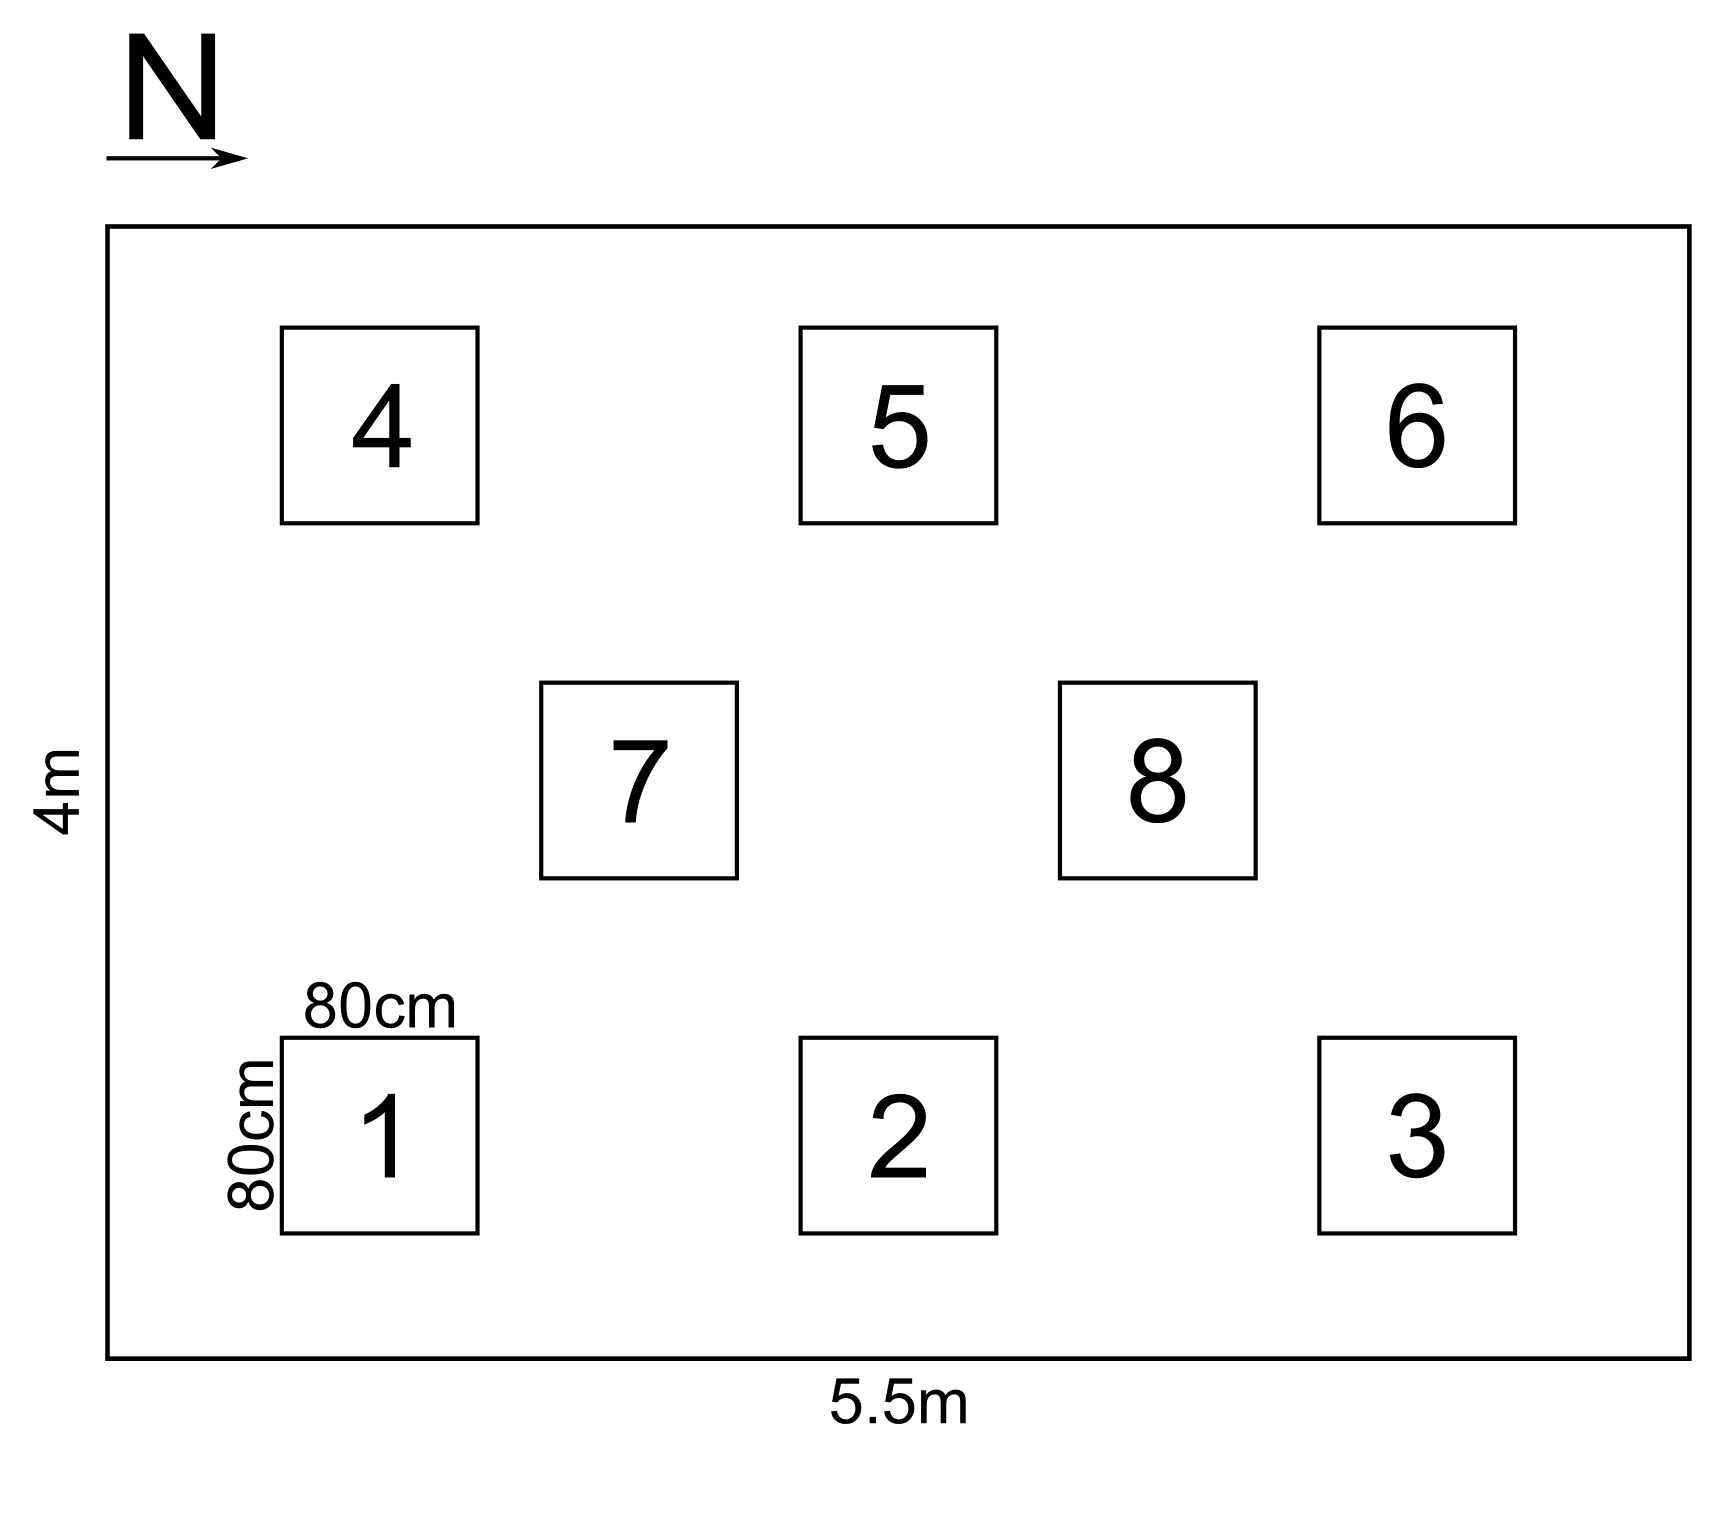
\includegraphics[width=9cm]{Images/plot-design}
 \caption{The sampling design within a plot}
 \label{fig:plot-design}
\end{figure}




\begin{itemize}
\item The pollinators were divided into bees, bumblebees, hoverflies and “other”
\item sampled eight of the 80x80cm patches per plot to get 2h of data per frequency and get a good mean over the plot (flowers were often in clusters and not distributed over the whole plot)
\item Patches were distributed as shown in Figure~\ref{fig:plot-design}
\end{itemize}

\begin{itemize}
\item When the flowers were very unevenly distributed over the Plot (which happened especially at low frequencies) I chose to observe some patches which contained flowers of the chosen species twice
\item I normally observed two species at once to save time/get a larger dataset. If there were not too many flowers that was easy feasible. If there were Plots with unevenly distributed flowers as explained above I observed the regular 1-8 patches for the evenly distributed species and additionally doubling patches for the uneven species. 
\item Eg. Geranium was flowering at all 8 patches, Lotus only in the southern part (patch 1,2,4,5, and 7). I regularly observed all patches 1-8 for Geranium. Because I was missing 3 patches for Lotus I doubled 1, 7 and 5. During this doubling I still kept track of visitors of the Geranium flowers. So in the end my dataset was the following:
\begin{itemize}
	\item 8+3 Geranium observations
	\item 8 Lotus observations
\end{itemize}
\end{itemize}


\subsection{Statistical Analysis}

\subsubsection{The Data}

Within the 4 weeks of sampling I got 386 entries, each equivalent to 15min of observation

\begin{itemize}
\item Flower visits to the focal species within the patch (divided by pollinator type)
\item Flower visits to other flowers except the focal species in the patch (divided by pollinator type)
\item Species Richness in the Patch (with names)
\item Species Richness in the Plot (with names and quantities)
\item Floral Cover in Patch and Plot (own estimation)
\item Frequency of the focal species in Patch and Plot
\item Count of individual flowers respectively inflorescence of the focal species
\item PlotID
\item PatchID
\item Date/Time
\end{itemize}


\subsection{The model}




  
